\section{Variational Analysis} \label{sec:variational}

For each tag-matching metric, we performed single-step mutational analyses to examine the local mutational neighborhood of loosely-affiliated and tightly-affiliated tag pairs and a mutational walk analysis to survey the broader mutational landscape.

\subsection{Single-Step Mutations}

\begin{figure}
\begin{center}

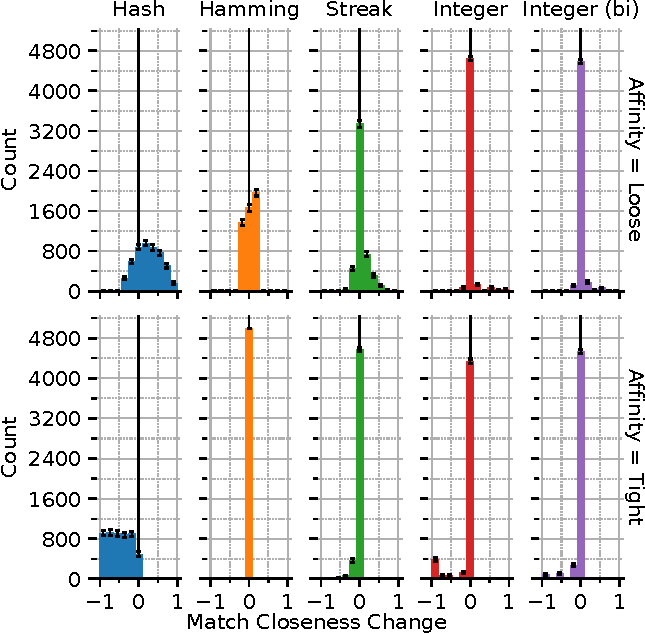
\includegraphics[width=\columnwidth]{img/mutational_step/bitweight=0dot5+seed=1+title=low-mutational-step+viz=hist+_data_hathash_hash=95a57768de56995a+_script_fullcat_hash=aa068ad24b386169+ext=}
\caption{
Distributions of mutation effects on match distance for loosely matched (pre-mutation match distance $> 0.5$) and tightly matched (pre-mutation match distance $< 0.01$) tag pairs.
Note that match closeness change (rather than mast distance change) is plotted so that better-matching mutational outcomes fall to the right and worse-matching mutational outcomes fall to the left.
Error bars are 95\% confidence intervals calculated using the Wilson score method with continuity correction \citep{newcombe1998two}.
Supplementary Figure \ref{fig:mutational_step_supp} shows the cumulative distribution of all sampled match distance changes for each metric.
}
\label{fig:mutational_step}

\end{center}
\end{figure}


Figure \ref{fig:mutational_step} visualizes the distribution of changes to match distance from single-bit mutations.

The distribution of mutational perturbations on loosely-affiliated tag pairs reflects the effects of one-step mutations on tags without pre-existing affinity.
To measure the distribution of mutational perturbations on loosely-affiliated tag pairs We began by sampling a target tag and then randomly sampled candidate tags until we found a second tag with a match distance $> 0.5$.
We recorded the match distance between our tag pair, applied a one-bit mutation to the secondary tag, and then measured the match distance between the tag pair again.
We repeated this process to generate 5000 samples.
Mutational perturbation was calculated as the difference between the match distances.
A negative mutational perturbation indicates a decrease in match distance and, therefore, an increase in match quality.

We measured the distribution of mutational perturbations on tightly-matched tag pairs similarly, except we uniformly sampled secondary candidate tags until we found a second tag with match distance $< 0.01$.
This distribution reflects the effects of one-step mutations on tags with pre-existing affinity.

For both tightly- and loosely-affiliated tag pairs under the integer and bidirectional integer metrics, most mutations caused very small changes in match distance.
These mutations toggle least-significant bits of the tag's integer representation.
However, under these metrics, a small fraction of mutations affecting more-significant bits of the integer representation have a much stronger effect.
Single-step mutations occasionally occur that strongly couple loosely-affiliated tag pairs or strongly decouple tightly-affiliated tag pairs.
In particular, the unidirectional integer metric appears to exhibit more frequent strong decoupling mutations than the bidirectional integer metric, presumably due to its non-commutative quirks.

The streak metric exhibits a large fraction of perfectly neutral outcomes under mutation.
These perfectly-neutral mutations presumably affect regions of the bitstring neither involved in the longest-matching streak nor in the longest-mismatching streak.
The streak metric exhibits a fatter tail of mutational magnitude for mutations that couple loosely-affiliated tags than the integer metrics. %TODO - consider word change for 'fatter'
In addition, the most extreme mutational outcomes that couple loosely-affiliated tags appear to be of a comparable magnitude to those under the integer metrics.
Mechanistically, this might be due to mutations that disrupt longest-mismatching streaks.
However, one-step mutations that decouple tightly-affiliated tags do not appear as potent.
This might be because achieving a very poor match requires both increasing longest-mismatching streak length and decreasing longest-matching streak length.

The hamming metric exhibits a generally uniform magnitude of match-distance changes under mutation.
High-magnitude one-step mutations do not occur under this metric.
(Without normalizing match distance to a uniform distribution for randomly-sampled tags, all hamming metric mutations would be of exactly the same magnitude, either increasing or decreasing the count of matching bits by 1.)

The hash metric exhibits the fattest tails of mutational magnitude of all metrics.
Extreme-effect one-step mutations are plentiful under this metric.
Interestingly, compared to other metrics, the hash metric exhibits a greater fraction of mutations that decouple tightly-affiliated tags and a greater fraction of mutations that couple loosely-affiliated tags.
This might be due to the hash metric's lack of geometric structure.
Because all one-step mutations uniformly sample a new match distance, 99\% of one-step mutations on tightly-affiliated tags will result in a looser coupling.
Similarly, approximately 75\% of one-step mutations on loosely-affiliated tags will result in a tighter coupling.

\subsection{Mutational Walks}

\begin{figure}
\begin{center}

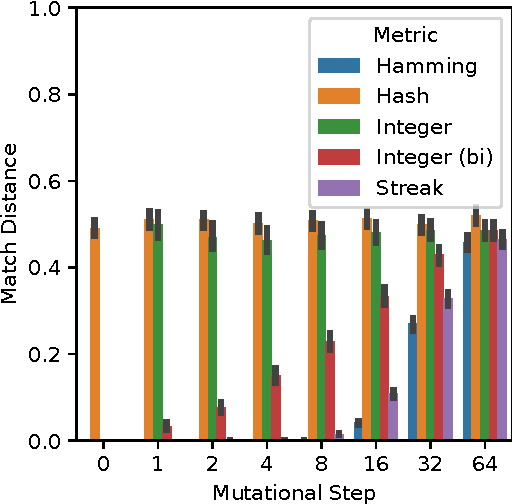
\includegraphics[width=\columnwidth]{{{mutational_walk/bitweight=0.5+seed=1+title=mutational_walk_barplot+_data_hathash_hash=8bf152d87daa9cb7+_script_fullcat_hash=982405ca713eba73+ext=}}}
\caption{
Snapshots of match distance at exponentially increasing steps from identical tags.
Error bars represent 95\% confidence intervals.
}
\label{fig:mutational_walk_barplot}

\end{center}
\end{figure}


Figure \ref{fig:mutational_walk_barplot} shows how match distance increases of mutational walks from initially exactly-equivalent tags.
%Match distances from each metric along these walks are compared side-by-side for exponentially-spaced mutational steps.
To conduct a mutational walk, we first randomly generated a starting tag.
Then, we sequentially applied 65 randomly-chosen one-step bit flip mutations, with back mutation allowed.
At each step along the walk, we measured match distance to the original starting tag.
We analyzed 1000 replicate mutational walks for each metric.

Under the hash metric, bitwise equivalent tags do not exhibit low match distance.
So, the mutational walk begins with and then maintains a mean match distance of 0.5.
Under the integer metric, half of mutational steps cause a wrap around effect, immediately spiking the average match distance to 0.5.
% Supplementary Figure \ref{fig:mutational_walk_lineplot} shows match distance variance decreasing as the walk proceeds away from match distances biased towards 0 or 1 \cite{Moreno_Ofria_2020}.
The bidirectional integer metric proceeds away from match distance 0 the next quickest, presumably due to large-effect mutations affecting significant bits. %TODO - added 'to' after '0' - confirm that sentence is correct
% - @AML: 'away from match distance 0 to the next quickest' => to what? I think 'to' breaks the sentence, removing.

The streak metric proceeds away from match distance 0 the second-slowest, trailed only by the hamming metric. %TODO - added 'to' after '0' - confirm that sentence is correct
% @AML: see above comment about 'to'
Interestingly, this result contradicts Downing's presentation of the streak metric in \citep{downing2015intelligence}, in which he suggests that the streak metric exhibits greater robustness because its match distance diverges more slowly under a mutational walk.
This discrepancy is presumably due to our normalization to ensure a uniform distribution of raw match scores between 0 and 1.


